\documentclass[letterpaper]{article} % DO NOT CHANGE THIS
\usepackage[submission]{aaai2027}  % DO NOT CHANGE THIS
% The serif, sans-serif, and monospaced fonts are loaded automatically by
% aaai2027.sty (newtxtext, helvet, courier). DO NOT add \usepackage{times},
% \usepackage{helvet}, \usepackage{courier}, or any other font package.
\usepackage[hyphens]{url}  % DO NOT CHANGE THIS
\usepackage{graphicx} % DO NOT CHANGE THIS
\urlstyle{rm} % DO NOT CHANGE THIS
\def\UrlFont{\rm}  % DO NOT CHANGE THIS
\usepackage{natbib}  % DO NOT CHANGE THIS AND DO NOT ADD ANY OPTIONS TO IT
\usepackage{caption} % DO NOT CHANGE THIS AND DO NOT ADD ANY OPTIONS TO IT
\frenchspacing  % DO NOT CHANGE THIS
%
% These are recommended to typeset algorithms but not required. See the subsubsection on algorithms. Remove them if you don't have algorithms in your paper.
\usepackage{algorithm}
\usepackage{algorithmic}

%
% These are recommended to typeset listings but not required. See the subsubsection on listing. Remove this block if you don't have listings in your paper.
\usepackage{newfloat}
\usepackage{listings}
\DeclareCaptionStyle{ruled}{labelfont=normalfont,labelsep=colon,strut=off} % DO NOT CHANGE THIS
\lstset{%
	basicstyle={\footnotesize\ttfamily},% footnotesize acceptable for monospace
	numbers=left,numberstyle=\footnotesize,xleftmargin=2em,% show line numbers, remove this entire line if you don't want the numbers.
	aboveskip=0pt,belowskip=0pt,%
	showstringspaces=false,tabsize=2,breaklines=true}
\floatstyle{ruled}
\newfloat{listing}{tb}{lst}{}
\floatname{listing}{Listing}

%
% Recommended for better-looking tables
\usepackage{booktabs}

%
% Keep the \pdfinfo as shown here. There's no need
% for you to add the /Title and /Author tags.
\pdfinfo{
/TemplateVersion (2027.1)
}

% DISALLOWED PACKAGES
% \usepackage{authblk} -- This package is specifically forbidden
% \usepackage{balance} -- This package is specifically forbidden
% \usepackage{CJK} -- This package is specifically forbidden
% \usepackage{float} -- This package is specifically forbidden
% \usepackage{flushend} -- This package is specifically forbidden
% \usepackage{fullpage} -- This package is specifically forbidden
% \usepackage{geometry} -- This package is specifically forbidden
% \usepackage{hyperref} -- This package is specifically forbidden
% \usepackage{navigator} -- This package is specifically forbidden
% (or any other package that embeds links such as navigator or hyperref)
% \usepackage{indentfirst} -- This package is specifically forbidden
% \usepackage{layout} -- This package is specifically forbidden
% \usepackage{multicol} -- This package is specifically forbidden
% \usepackage{nameref} -- This package is specifically forbidden
% \usepackage{savetrees} -- This package is specifically forbidden
% \usepackage{setspace} -- This package is specifically forbidden
% \usepackage{stfloats} -- This package is specifically forbidden
% \usepackage{tabu} -- This package is specifically forbidden
% \usepackage{titlesec} -- This package is specifically forbidden
% \usepackage{tocbibind} -- This package is specifically forbidden
% \usepackage{ulem} -- This package is specifically forbidden
% \usepackage{wrapfig} -- This package is specifically forbidden
% DISALLOWED COMMANDS
% \nocopyright -- Your paper will not be published if you use this command
% \addtolength -- This command may not be used
% \balance -- This command may not be used
% \baselinestretch -- Your paper will not be published if you use this command
% \clearpage -- No page breaks of any kind may be used for the final version of your paper
% \columnsep -- This command may not be used
% \newpage -- No page breaks of any kind may be used for the final version of your paper
% \pagebreak -- No page breaks of any kind may be used for the final version of your paper
% \pagestyle -- This command may not be used
% \tiny -- This is not an acceptable font size.
% \vspace{- -- No negative value may be used in proximity of a caption, figure, table, section, subsection, subsubsection, or reference
% \vskip{- -- No negative value may be used to alter spacing above or below a caption, figure, table, section, subsection, subsubsection, or reference

\setcounter{secnumdepth}{0} %May be changed to 1 or 2 if section numbers are desired.

% The file aaai2027.sty is the style file for AAAI Press
% proceedings, working notes, and technical reports.
%

% Title

% Your title must be in mixed case, not sentence case.
% That means all verbs (including short verbs like be, is, using,and go),
% nouns, adverbs, adjectives should be capitalized, including both words in hyphenated terms, while
% articles, conjunctions, and prepositions are lower case unless they
% directly follow a colon or long dash
\title{DREAMRec: Denoised and Decoupled Retrieval with Adaptive Memory for Sequential Recommendation}
\author{
    %Authors
    % All authors must be in the same font size and format.
    Written by AAAI Press Staff\textsuperscript{\rm 1}\thanks{With help from the AAAI Publications Committee.}\\
    AAAI Style Contributions by Peter Patel Schneider,
    Sunil Issar,\\
    J. Scott Penberthy,
    George Ferguson,
    Hans Guesgen,
    Francisco Cruz\equalcontrib\corresponding,
    Marc Pujol-Gonzalez\equalcontrib\corresponding
}
\affiliations{
    %Afiliations
    \textsuperscript{\rm 1}Association for the Advancement of Artificial Intelligence\\
    % If you have multiple authors and multiple affiliations
    % use superscripts in text and roman font to identify them.
    % For example,

    % Sunil Issar\textsuperscript{\rm 2},
    % J. Scott Penberthy\textsuperscript{\rm 3},
    % George Ferguson\textsuperscript{\rm 4}\corresponding,
    % Hans Guesgen\textsuperscript{\rm 5}
    % Note that the comma should be placed after the superscript

    1101 Pennsylvania Ave, NW Suite 300\\
    Washington, DC 20004 USA\\
    % email address must be in roman text type, not monospace or sans serif
    proceedings-questions@aaai.org
%
% See more examples next
}

%Example, Single Author, ->> remove \iffalse,\fi and place them surrounding AAAI title to use it
\iffalse
\title{My Publication Title --- Single Author}
\author {
    Author Name
}
\affiliations{
    Affiliation\\
    Affiliation Line 2\\
    name@example.com
}
\fi

\iffalse
%Example, Multiple Authors, ->> remove \iffalse,\fi and place them surrounding AAAI title to use it
\title{My Publication Title --- Multiple Authors}
\author {
    % Authors
    First Author Name\textsuperscript{\rm 1,\rm 2}\equalcontrib,
    Second Author Name\textsuperscript{\rm 2}\equalcontrib,
    Third Author Name\textsuperscript{\rm 1}\corresponding
}
\affiliations {
    % Affiliations
    \textsuperscript{\rm 1}Affiliation 1\\
    \textsuperscript{\rm 2}Affiliation 2\\
    firstAuthor@affiliation1.com, secondAuthor@affilation2.com, thirdAuthor@affiliation1.com
}
\fi


\usepackage{amsthm}  % 如果用的是 ACM 模板，通常自带这个，可以不加这行，但加了也不报错
\usepackage{amsmath}
\usepackage{amssymb}

% 定义 definition 环境
\theoremstyle{definition} % 这一行很重要！让定义的内容变成正体字，而不是斜体
\newtheorem{definition}{Definition}

\newcommand{\mypara}[1]{\vspace{8pt}\noindent\textbf{#1}}
\usepackage{bm}
\usepackage{multirow}

\begin{document}

\maketitle

\begin{abstract}
Sequential Recommender Systems aim to capture dynamic user preferences by mining historical dependencies. However, existing methods typically adopt a truncation strategy that focuses mainly on the most recent interactions. From a cognitive psychology perspective, real-world user behavior is jointly driven by immediate intent and accumulated historical habits. The truncation strategy ignores information in the dimension of historical preferences and is limited entirely to recent information. A straightforward solution is to feed the user’s
entire historical sequence into the model. However, as the sequence length increases, the attention weights for each item are diluted. The dilution confronts two critical challenges: amplified noise interference and the inability to focus on specific regularities. To address these issues, we propose \textbf{DHPRec} (\underline{D}enoised \underline{H}istorical \underline{P}atterns for Sequential \underline{Rec}ommendation), a novel framework designed to bridge immediate intent and specific long-term patterns. DHPRec introduces a Frequency-Domain Feature Refinement mechanism to filter high-frequency noise and extract stable long-term representations. Furthermore, we design a Pattern-Based Anchor-Guided Fusion mechanism,which extracts pattern units representing long-term regularities and utilizes an anchor to effectively extract the global specific historical preferences. 
\end{abstract}

% Uncomment the following to link to your code, datasets, an extended version or similar.
% You must keep this block between (not within) the abstract and the main body of the paper.
% Make sure that you do not de-anonymize yourself with these links.
% \begin{links}
%     \link{Code}{https://aaai.org/example/code}
%     \link{Datasets}{https://aaai.org/example/datasets}
%     \link{Extended version}{https://aaai.org/example/extended-version}
% \end{links}

\section{Introduction}

Sequential recommendation aims to predict users' next behaviors based on their historical interactions and has become an essential component in real-world applications, such as e-commerce, short-video platforms, and news recommendation systems. With the growing number of users and the increasing diversity of item content, user behavior sequences have become more complex and heterogeneous. Therefore, how to accurately capture users' interests from complex historical interactions remains a fundamental challenge in sequential recommendation.

Recently, the rapid development of pre-trained language models has driven increasing efforts to leverage textual descriptions of items for semantic representation learning, shifting sequential recommendation from traditional ID-based representations toward semantic-aware modeling. Existing methods typically feed item semantic representations into sequential encoders, such as CNNs, RNNs, and Transformers, to learn a unified user representation from historical interactions, which is then matched with candidate items for ranking. This paradigm of "item semantic encoding–sequential representation learning–user representation matching" has become a prevalent framework in modern sequential recommendation.

However, user historical behaviors inherently contain diverse types of information, including behavioral noise, long-term preferences, and short-term emerging intents. Existing unified user modeling approaches usually compress these heterogeneous signals into a single representation, which may cause interference among different interest patterns and limit the model's ability to accurately characterize users' true preferences. Specifically, existing methods still face the following three challenges.

\begin{figure}[t]
    \centering    
    % 第一张图
    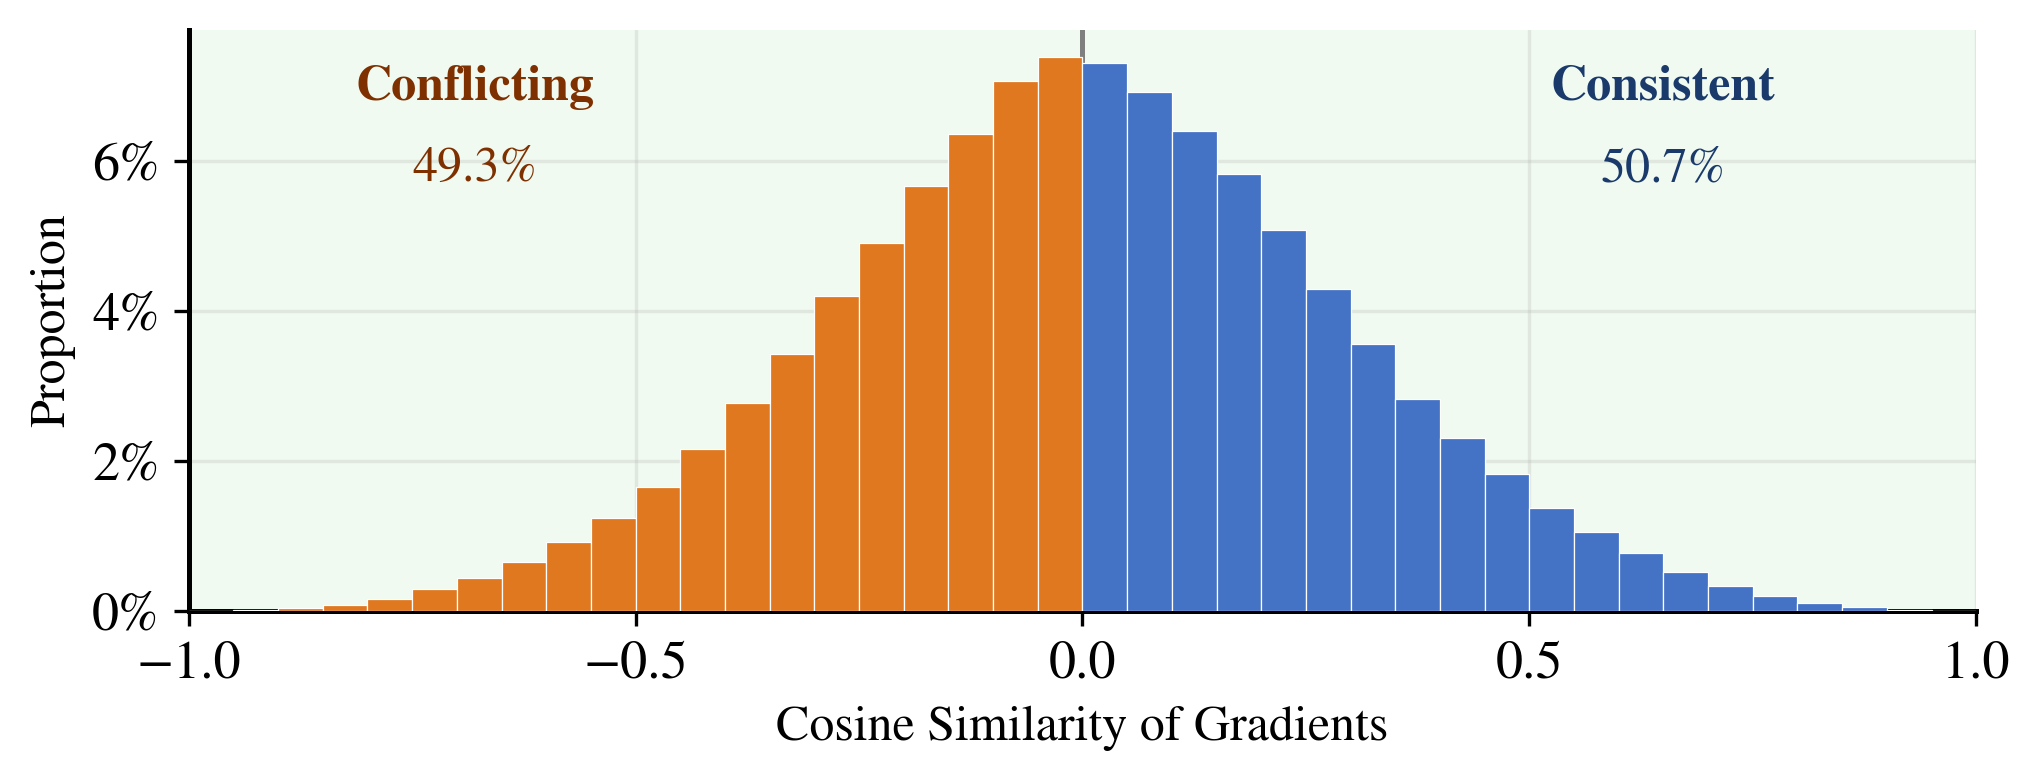
\includegraphics[width=1\linewidth]{fig2_grad_conflict.png}
    \caption{Distribution of Gradient Conflicts between Retrieval and Prediction Tasks.}
    \label{fig:spectrum}
\end{figure}

The first challenge lies in distinguishing behavioral noise from genuine interests. User historical behaviors simultaneously contain various signals, including genuine preferences, exploratory behaviors, and random noise. Existing denoising methods typically assume that high-frequency signals correspond to noise and suppress them accordingly. However, high-frequency components may also reflect users' genuine bursty interests, such as a strong short-term demand for a new category that appears intensively within a short period. Therefore, directly filtering such signals may remove valuable behaviors, making it difficult for models to accurately distinguish noise from true interests.

The second challenge is the lack of dynamic coordination between short-term and long-term interests. Users' next behaviors are usually driven jointly by long-term stable preferences and short-term immediate needs. Existing methods mainly model different temporal scales implicitly through truncation strategies, attention mechanisms, or hierarchical structures. However, massive repetitive and sparse interactions may obscure core preference patterns, making it difficult to form stable and structured memories. Moreover, when long-term preferences conflict with recent needs, such as a user with a long-term preference for sports suddenly becoming interested in cooking, existing models lack the ability to perceive the current context and dynamically determine which interest should dominate. Therefore, how to dynamically balance different interests while consolidating long-term memory remains an open challenge.

The third challenge is the representation bottleneck caused by unified user representations. Existing methods typically compress user historical behaviors into a single representation, which is then simultaneously used for historical retrieval and recommendation prediction. However, retrieval requires the representation to preserve similarity with historical behaviors, whereas prediction requires the representation to maintain sufficient discriminative capability for distinguishing candidate items. These two objectives are inherently inconsistent. When a single representation is optimized for both tasks simultaneously, conflicts between objectives may arise, limiting the expressive capability of user representations. As shown in Figure 1, on the ML-1M dataset, approximately 49.3\% of samples exhibit conflicting gradient directions between the retrieval objective and the prediction objective (cosine similarity < 0), indicating that unified representation learning is indeed affected by interference from different optimization objectives.

To address the above three challenges, we propose DREAMRec (Denoised and Decoupled Retrieval with Adaptive Memory for Recommendation), an adaptive memory modeling framework for sequential recommendation. DREAMRec progressively refines user representations through three stages: behavior denoising, semantic memory construction, and decoupled retrieval. Specifically, we first introduce a Wavelet-Enhanced Burstiness-preserving Denoiser (WEBD), which suppresses behavioral noise while preserving genuine interest signals. Then, we develop a Semantic Memory Prototyping module (SMP) to organize denoised historical behaviors into compact long-term semantic memories, and further incorporate context-aware queries to dynamically coordinate short-term and long-term interests. Finally, we design a Decoupled Memory Retrieval module (DMR), which performs memory matching and user representation learning in separate retrieval and representation spaces, alleviating the objective conflicts caused by unified representation learning. Through these designs, DREAMRec progressively achieves behavior refinement, interest organization, and retrieval optimization, effectively reducing the interference among heterogeneous interest signals and enabling more accurate and robust user modeling.

The main contributions of this paper are summarized as follows:

\begin{itemize}
    \item We propose DREAMRec, an adaptive memory modeling framework for sequential recommendation, which enables more refined user interest modeling through behavior denoising, semantic memory construction, and decoupled retrieval.

    \item We design a wavelet-enhanced denoising mechanism that preserves bursty interests, along with a memory modeling approach based on semantic prototypes and decoupled retrieval, effectively improving the robustness and discriminability of user representations.

    \item Extensive experiments on multiple public benchmarks demonstrate that DREAMRec consistently outperforms state-of-the-art methods, and ablation studies further validate the effectiveness of each proposed component.
\end{itemize}

\section{Method}
\subsection{Problem Formulation}

Let $\mathcal{U}=\{u_1,\cdots,u_{|\mathcal U|}\}$ and $\mathcal{V}=\{v_1,\cdots,v_{|\mathcal V|}\}$ denote the user set and the item set, respectively. Each item $v\in\mathcal V$ is associated with a unique item ID as well as a set of textual attributes, such as the product title, brand, and category. To leverage semantic information, we employ a semantic encoder to obtain the semantic representation of each item, denoted by $\bm{z}_i\in\mathbb{R}^{d}$, where $d$ is the embedding dimension.

For each user, the historical interaction sequence is represented as $\mathcal{S}=\{v_1,\cdots,v_L\}$, and the corresponding sequence of semantic representations is denoted by $\bm{Z}=[\bm{z}_1,\cdots,\bm{z}_L]$. Given the historical interaction sequence $\mathcal{S}$, the objective of sequential recommendation is to predict the next item that the user is most likely to interact with, i.e., maximizing the conditional probability:$P(v_{L+1}\mid\mathcal S).$
\begin{figure*}[t]  % <--- 注意这里变成了 figure*，[t] 表示优先放页顶
  \centering        % 建议加上居中，否则图片可能偏左
  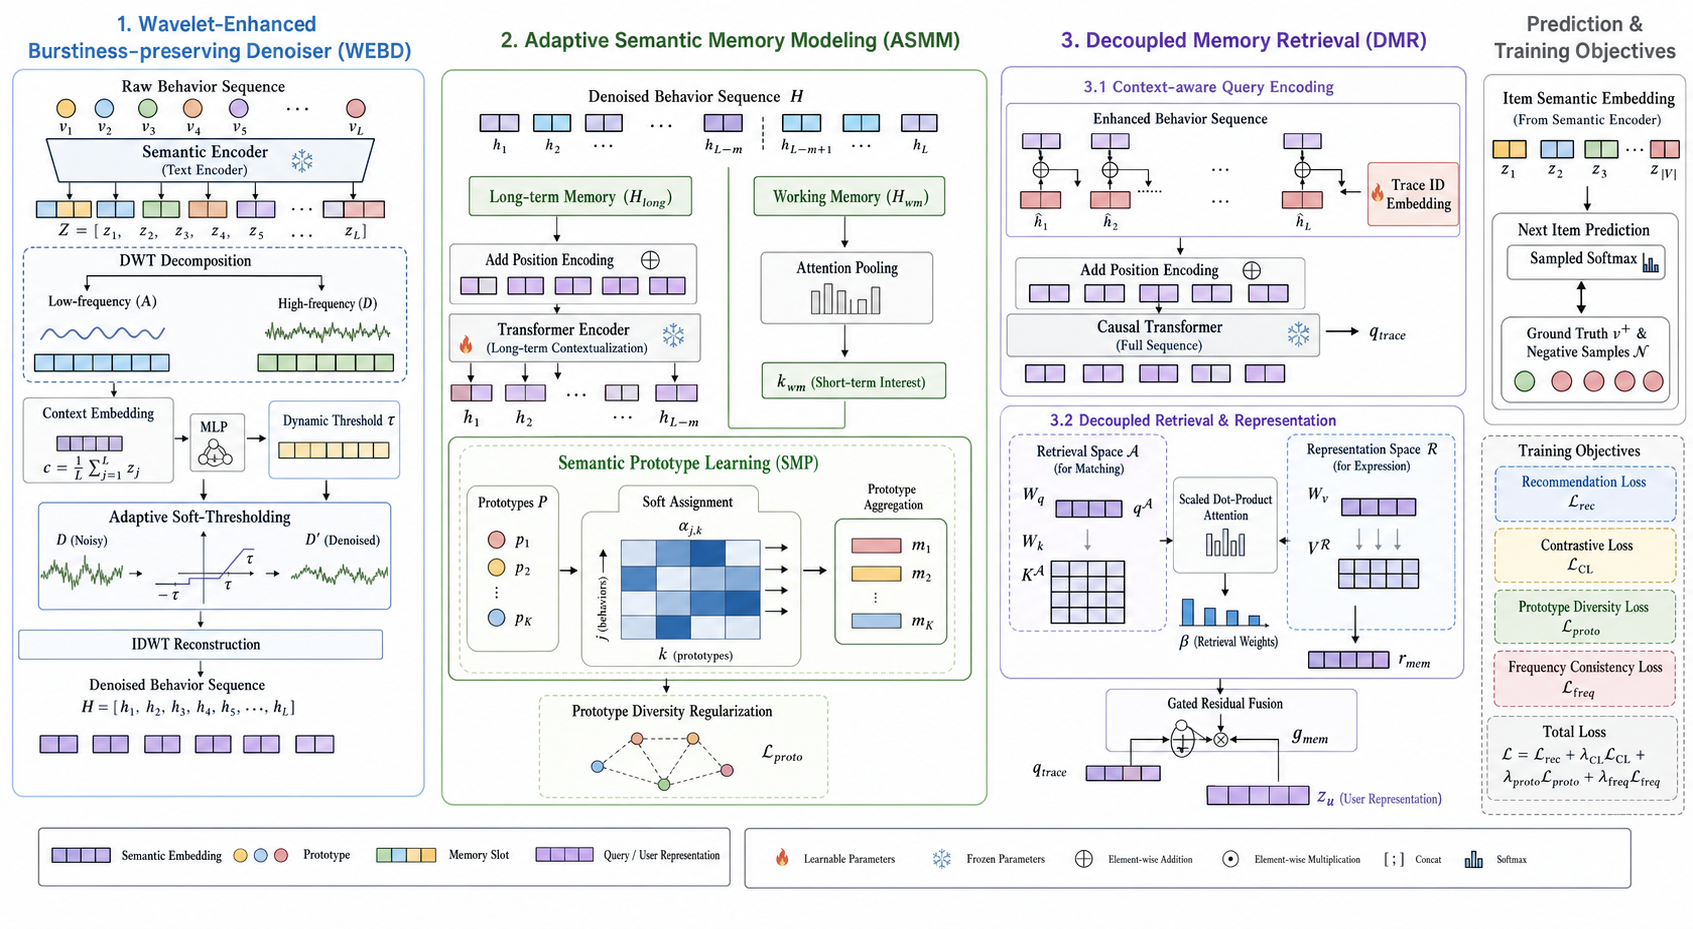
\includegraphics[width=\textwidth]{fracwork.png} % 这里 width=\textwidth 代表整个页面的宽度
\caption{The overall architecture of DHPRec. (Bottom) The Frequency-Domain Feature Refinement module constructs refined item representations via spectral denoising. 
(Middle) The Pattern-Based Anchor-Guided Fusion Network, which transforms the sequence into compact Pattern Units and utilizes the Anchor to extract relevant long-term regularities.  
(Top) A motivating example illustrating how the Immediate Intent (e.g., Christmas demand) bridges specific Historical Habits. }


    \label{fig:framework}
  \label{fig:teaser}
\end{figure*}
\subsection{Wavelet-Enhanced Burstiness-preserving Denoiser}

High-frequency variations in user behavior sequences may originate from either random noise or genuine bursty interests. Existing frequency-based denoising methods usually suppress high-frequency components uniformly, which may remove informative signals reflecting emerging user preferences. To address this issue, we propose the Wavelet-Enhanced Burstiness-preserving Denoiser (WEBD), which refines behavior representations by suppressing noise while preserving meaningful bursty patterns.

Specifically, WEBD decomposes the behavior sequence into low-frequency trends and high-frequency details via wavelet transform, and learns context-aware thresholds to selectively suppress noisy variations while retaining informative high-frequency signals. The refined sequence is then reconstructed through inverse wavelet transform, providing reliable behavior representations for subsequent semantic memory modeling.

\subsubsection{Behavior Decomposition}

Given the user behavior representation sequence  $\bm{Z}=[\bm{z}_1,\bm{z}_2,\cdots,\bm{z}_L]$,WEBD performs multi-scale decomposition using the Discrete Wavelet Transform (DWT):
\begin{equation}
\bm{A}, \bm{D} = \text{DWT}(\bm{Z}),
\end{equation}
where $\bm{A}$ and $\bm{D} \in \mathbb{C}^{(L' + 1) \times d}$, $L'=\lfloor L /2 \rfloor$. Here, $\bm{A}$ and $\bm{D}$ denote the low-frequency trend and high-frequency detail components, respectively. The low-frequency component captures stable interest evolution, while the high-frequency component reflects local behavioral changes. Since high-frequency variations may represent either noise or genuine bursty interests, adaptive discrimination is required.

\subsubsection{Adaptive Burst-preserving Denoising}

We learn context-dependent thresholds from the entire behavior sequence. Specifically, a global contextual representation is obtained by average pooling:
\begin{equation}
\bm{c} = \frac{1}{L}\sum_{j=1}^{L}\bm{z}_j.
\end{equation}

The contextual representation is then fed into a lightweight MLP to predict channel-wise adaptive thresholds:
\begin{equation}
\boldsymbol{\tau} = \alpha \cdot \sigma\left(\text{MLP}\!\left(\bm{c}\right)\right),
\end{equation}
where $\alpha$ is a learnable scaling factor and $\sigma(\cdot)$ denotes the sigmoid function. Given the learned thresholds, soft-thresholding is applied to the high-frequency coefficients:
\begin{equation}
\bm{D}' = \text{sign}(\bm{D}) \cdot \max(|\bm{D}|-\boldsymbol{\tau},0).
\end{equation}

The adaptive threshold mechanism adjusts the denoising strength according to behavioral contexts. Smaller thresholds preserve consistent high-frequency patterns corresponding to bursty interests, while larger thresholds suppress irregular fluctuations caused by noise.

\subsubsection{Behavior Reconstruction}

Finally, the refined high-frequency components are combined with the low-frequency trends and reconstructed through the Inverse Discrete Wavelet Transform (IDWT):
\begin{equation}
\bm{H} = \text{IDWT}(\bm{A},\bm{D}').
\end{equation}

The reconstructed sequence is represented as $\bm{H}=[\bm{h}_1,\bm{h}_2,\cdots,\bm{h}_L]$. By selectively removing random fluctuations while preserving stable trends and bursty interests, WEBD provides cleaner inputs for subsequent semantic memory modeling.

\subsection{Adaptive Semantic Memory Modeling}

Although WEBD refines behavior representations, the resulting sequence still mixes short-term intentions and long-term preferences. To explicitly model interests across different temporal scales, we propose Adaptive Semantic Memory Modeling, which organizes user behaviors into a hierarchical memory structure. Specifically, recent interactions are preserved as Working Memory for capturing immediate interests, while long-term behaviors are compressed into Semantic Prototypes to construct compact and retrievable semantic memories.

\subsubsection{Memory Construction}

Given the refined behavior sequence from WEBD, $\bm{H}=[\bm{h}_1,\bm{h}_2,\cdots,\bm{h}_L],$ To capture user interests at different temporal scales, we divide the sequence into working memory and long-term memory according to a ratio $\rho$: $\bm{H}_{short}=
[\bm{h}_{L-\lfloor\rho L\rfloor+1},\cdots,\bm{h}_{L}],\ 
\bm{H}_{long}=
[\bm{h}_{1},\cdots,\bm{h}_{L-\lfloor\rho L\rfloor}]$. 

The working memory captures recent user intentions, while the long-term memory models stable preference patterns. For each representation $[\bm{H}_{short}]_j$, where $j \in \{1,\ldots,|\bm{H}_{short}|\}$, we obtain the short-term interest: \begin{equation}
a_j=\text{softmax}(\bm{w}_a^\top[\bm{H}_{wm}]_j),
\end{equation}
\begin{equation}
\bm{s}=\sum_{j=1}^{|\bm{H}_{short}|}a_j[\bm{H}_{short}]_j.
\end{equation}
where $\mathbf{w}_a$ is a learnable attention vector. The resulting $\bm{s}_{wm}$ serves as the short-term interest representation for subsequent memory retrieval.

\subsubsection{Semantic Prototype Learning}

Directly retaining all historical behaviors introduces redundancy and makes it difficult to form reusable long-term memories. Therefore, we compress long-term behaviors into a set of semantic prototypes. We maintain $K$ learnable semantic prototypes $\bm{P}=[\bm{p}_1,\ldots,\bm{p}_K]\in\mathbb{R}^{K\times d}$. For the long-term memory $\bm{H}_{long}$, positional embeddings and a Transformer encoder are applied to capture temporal dependencies:
\begin{equation}
\widetilde{\bm{H}}_{long}=\text{Transformer}(\text{LN}(\bm{H}_{long}+\bm{P}_{long})).
\end{equation}
where $\bm{P}_{long}$ denotes the learnable positional embeddings. For each contextualized behavior representation $\widetilde{\bm{h}}_j$, its assignment probability over prototypes is computed as:
\begin{equation}
\alpha_{j,k}=
\frac{\exp(\widetilde{\bm{h}}_j^\top\bm{p}_k/\tau_p)}
{\sum_{l=1}^{K}\exp(\widetilde{\bm{h}}_j^\top\bm{p}_l/\tau_p)}.
\end{equation}
where $\tau_p$ is a temperature coefficient controlling the sharpness of prototype assignments. Then the $k$-th semantic memory slot is obtained by weighted aggregation:
\begin{equation}
\bm{m}_k=
\frac{\sum_j\alpha_{j,k}\widetilde{\bm{h}}_j}
{\sum_j\alpha_{j,k}+\epsilon}.
\end{equation}
where $\epsilon$ is a small constant for numerical stability. The resulting long-term semantic memory is $\bm{M}_{long}=[\bm{m}_1,\ldots,\bm{m}_K]\in\mathbb{R}^{K\times d}$. By converting numerous historical interactions into a small number of semantic prototypes, the model obtains compact long-term memories that can be dynamically retrieved under different recommendation contexts.

Finally,together with the aggregated working memory representation, the complete user memory is formulated as:
\begin{equation}
\bm{M}=[\mathbf{M}_{long};\mathbf{s}] 
\end{equation}
\subsubsection{Prototype Diversity Regularization}

To prevent semantic prototypes from collapsing into similar representations, we introduce a diversity regularization term:
\begin{equation}
 \mathcal{L}{ortho} = \frac{1}{K}\sum_{k=1}^{K} \max_{ j\neq k} \cos(\mathbf{p}_k, \mathbf{p}_j),
\end{equation}
where $\cos(\cdot,\cdot)$ denotes cosine similarity. This constraint encourages different memory slots to capture complementary interest patterns.

\subsection{Decoupled Memory Retrieval}

After constructing the hierarchical memory structure, we obtain a user memory representation consisting of working memory and long-term semantic memory. To exploit these memories under different recommendation contexts, the model needs to dynamically retrieve relevant long-term interests according to the current behavioral trajectory.

However, existing sequential recommendation methods typically employ a unified representation space for both memory retrieval and final prediction, where similarity matching and semantic discrimination are optimized simultaneously. Such a design may introduce representation conflicts. To address this issue, we propose Decoupled Memory Retrieval (DMR), which separates memory retrieval and semantic representation learning into two independent spaces. Specifically, DMR first constructs a context-aware query from the complete behavioral trajectory to retrieve relevant semantic memories, and then projects the retrieved information into a dedicated representation space for recommendation prediction.


\subsubsection{Context-aware Query Encoding}

To capture the current recommendation context, we construct a query from the complete behavioral trajectory rather than only recent interactions. However, semantic item representations may lack sufficient discrimination when different items share similar meanings. Therefore, we introduce an independent Trace ID embedding table in the retrieval branch: $\bm{E} \in \mathbb{R}^{|\mathcal V| \times d}.$ For item $i$, its Trace ID representation is obtained as: $\bm{e}_i=\bm{E}[i].$

We inject the Trace ID information into the denoised behavior representation through a gated residual mechanism:
\begin{equation}
g_i = \sigma\!\left(\bm{W}_g[\bm{h}_i;\bm{e}_i]+b_g\right),
\end{equation}
\begin{equation}
\hat{\bm{h}}_i
=
\text{LN}(\bm{h}_i+g_i\odot\bm{e}_i),
\end{equation}
where $\bm{h}_i$ denotes the behavior representation produced by WEBD. The trajectory-enhanced sequence is formulated as: $\hat{\bm{H}}
=
[\hat{\bm{h}}_1,\hat{\bm{h}}_2,\cdots,\hat{\bm{h}}_L]$. After adding positional embeddings, a causal Transformer is applied:
\begin{equation}
\bm{H}_{trace}
=
\text{CausalTransformer}
(\hat{\bm{H}}+\bm{P}_{trace}).
\end{equation}
where $\bm{P}_{trace}$ denotes the learnable positional embeddings. The hidden state at the last position is projected to obtain the context-aware query: $\bm{q}_{trace}=\bm{W}_{q}\bm{H}_{trace}[L]$.

This query integrates both long-term behavioral patterns and recent intentions, providing a comprehensive context representation for memory retrieval.


\subsubsection{Decoupled Retrieval and Representation}

Given the context-aware query $\bm{q}_{trace}$, DMR retrieves relevant memories from the unified memory bank $\bm{M}$. 
We argue that memory matching and semantic representation learning optimize different objectives. 
Therefore, DMR explicitly separates these two processes into a Retrieval Space $\mathcal{A}$ and a Representation Space $\mathcal{R}$.

The retrieval space is responsible for measuring the relevance between the current context and historical memories.
The memory bank are first projected into the retrieval space:
\begin{equation}
\bm{M}^{\mathcal{A}}
=
\bm{W}_{m}^{\mathcal{A}}
\bm{M},
\end{equation}
where $\bm{W}_{m}^{\mathcal{A}}$ are learnable projection matrices. 
The retrieval weights are then computed according to the similarity between the context query and memory slots:
\begin{equation}
\boldsymbol{\beta}
=
\text{softmax}
\left(
\frac{
\bm{M}^{\mathcal{A}}
(\bm{q}^{\mathcal{A}})^{\top}
}
{\sqrt{d_a}}
\right),
\end{equation}

The retrieval space only determines which memories should be selected and does not directly participate in user representation learning. 
To preserve semantic information for recommendation prediction, the memory bank is independently projected into the representation space:
\begin{equation}
\bm{M}^{\mathcal{R}}
=
\bm{W}_{m}^{\mathcal{R}}
\bm{M},
\end{equation}
where $\bm{W}_{m}^{\mathcal{R}}$ denotes the representation projection matrix. The retrieved memory representation is obtained by aggregating memory slots according to the retrieval weights:
\begin{equation}
\bm{r}_{mem}
=
\boldsymbol{\beta}
\bm{M}^{\mathcal{R}}.
\end{equation}

Finally, we combine the retrieved long-term interests with the current behavioral context through gated residual~learning:
\begin{equation}
\bm{g}_{mem}
=
\sigma
(
\bm{W}_{g}
[\bm{q}_{trace};\bm{r}_{mem}]
+b_g
),
\end{equation}
\begin{equation}
\bm{z}_{u}
=
\text{LN}
(
\bm{q}_{trace}
+
\bm{g}_{mem}\odot\bm{r}_{mem}
).
\end{equation}

By decoupling retrieval and representation spaces, DMR allows memory matching and semantic prediction to be optimized independently. 
This design avoids the interference caused by conflicting objectives in unified representations and produces a more expressive user representation with adaptive coordination between short-term intentions and long-term preferences.
\subsection{Training Objective}

DREAMRec is trained in an end-to-end manner by jointly optimizing the recommendation objective and auxiliary regularization objectives. Specifically, we consider next-item prediction loss, contrastive learning loss, semantic prototype diversity regularization, and frequency consistency regularization.


\subsubsection{Recommendation Loss}

Given the learned user representation $\bm{z}_u$, we adopt sampled softmax cross-entropy for next-item prediction. Given the positive item $v^{+}$ and sampled negative items $\mathcal{N}$, the recommendation loss is defined as:

\begin{equation}
\mathcal{L}_{rec}
=
-\log
\frac{
\exp(s(u,i^+)/\tau)
}
{
\exp(s(u,i^+)/\tau)
+
\sum_{i^-\in\mathcal{N}}
\exp(s(u,i^-)/\tau)
},
\end{equation}
where $s(u,v)=\bm{z}_u^T\bm{z}_v$ denotes the matching score between user and item representations, and $\tau$ is the temperature coefficient.


\subsubsection{Contrastive Learning Objective}

To improve the robustness of user representations against behavioral perturbations, we introduce a contrastive learning objective. For each user sequence, a perturbed view is generated by randomly masking historical interactions, and the corresponding user representation $\widetilde{\bm{z}}_u$ is obtained using the same encoder.

We adopt a symmetric InfoNCE objective, treating different views of the same user as positive pairs and other users within the mini-batch as negative samples:
\begin{equation}
\mathcal{L}_{CL}
=
-\frac{1}{2}
(\mathcal{L}_{u\rightarrow \tilde{u}}
+
\mathcal{L}_{\tilde{u}\rightarrow u}),
\end{equation}
where $
\mathcal{L}_{u\rightarrow \tilde{u}}
=
-\log
\frac{
\exp(
\langle
\hat{\bm z}_u,
\hat{\tilde{\bm z}}_u
\rangle/\tau)
}
{
\sum_{j\in\mathcal{B}}
\exp(
\langle
\hat{\bm z}_u,
\hat{\tilde{\bm z}}_j
\rangle/\tau)
},
$
and $\mathcal{L}_{\tilde{u}\rightarrow u}$ is defined symmetrically. Here,
$\hat{\bm z}=\bm z/\|\bm z\|_2$ denotes the normalized representation and $\mathcal{B}$ represents the mini-batch user set.


\subsubsection{Overall Objective}

The final optimization objective is formulated as:
\begin{equation}
\mathcal{L}
=
\mathcal{L}_{rec}
+
\lambda_{CL}\mathcal{L}_{CL}
+
\lambda_{proto}\mathcal{L}_{proto}
\end{equation}
where $\lambda_{CL}$ and $\lambda_{proto}$ balance the contributions of the auxiliary objectives.

\begin{table*}[t]
  \centering
  \small % 严格遵守 AAAI 要求，使用 9pt 字体
  \setlength{\tabcolsep}{0.7mm} % 将列间距收紧到 0.9mm，足以消除溢出且不拥挤
  \renewcommand{\arraystretch}{1.2}

  % 注意开头和结尾的 @{}，这会直接砍掉表格最左侧和最右侧的默认留白，为你额外争取宝贵的水平空间
  \begin{tabular}{@{} l cccc cccc cccc cccc @{}}
    \toprule
    % --- 表头第一行 ---
    \multirow{2}{*}{Methods} &
    \multicolumn{4}{c}{Baby} &
    \multicolumn{4}{c}{Game} &
    \multicolumn{4}{c}{Scientific} &
    \multicolumn{4}{c}{ML-1M} \\

    \cmidrule(lr){2-5} \cmidrule(lr){6-9} \cmidrule(lr){10-13} \cmidrule(lr){14-17}

    % --- 表头第二行 ---
     & R@5 & R@10 & N@5 & N@10 & R@5 & R@10 & N@5 & N@10 & R@5 & R@10 & N@5 & N@10 & R@5 & R@10 & N@5 & N@10 \\

    \midrule
    % --- 第一组基线 ---
    BERT4Rec & 1.76 & 3.05 & 1.21 & 1.49 & 4.65 & 7.30 & 3.03 & 3.81 & 1.91 & 2.91 & 1.24 & 1.50 & 13.93 & 24.18 & 9.64 & 12.64 \\
    GRU4Rec  & 2.25 & 3.49 & 1.45 & 1.79 & 5.35 & 8.15 & 3.55 & 4.38 & 2.35 & 3.69 & 1.53 & 1.89 & 13.16 & 21.54 & 7.25 & 9.52 \\
    SASRec   & 2.16 & 3.57 & 1.40 & 1.75 & 5.40 & 8.52 & 3.36 & 4.33 & 2.64 & 4.07 & 1.55 & 1.94 & 14.05 & 23.00 & 8.74 & 11.46 \\
    FMLPRec  & 2.33 & 3.62 & 1.51 & 1.85 & 5.23 & 8.62 & 3.43 & 4.39 & 2.64 & 4.17 & 1.60 & 1.99 & 14.14 & 23.63 & 9.41 & 12.34 \\
    FDSA     & 2.38 & 3.92 & 1.63 & 2.00 & 5.49 & 8.57 & 3.56 & 4.65 & 2.68 & 4.21 & 1.78 & 2.24 & 13.97 & 22.86 & 8.92 & 11.70 \\
    % --- 第二组基线 ---
    S$^3$Rec & 2.21 & 3.33 & 1.31 & 1.73 & 4.90 & 7.74 & 3.20 & 4.11 & 2.58 & 4.23 & 1.76 & 2.14 & 13.86 & 22.68 & 8.68 & 11.38 \\
    DuoRec   & 2.06 & 3.51 & 1.44 & 1.77 & 5.64 & 8.49 & 3.73 & 4.64 & 2.50 & 3.84 & 1.61 & 2.14 & 14.17 & 22.81 & 9.68 & 11.17 \\
    MAERec   & 2.19 & 3.75 & 1.41 & 1.88 & 6.23 & 9.31 & 4.06 & 5.08 & 2.98 & 4.57 & 2.10 & 2.48 & 13.97 & 23.45 & 9.42 & 11.65 \\
    % --- 第三组基线 ---
    UniSRec  & 2.34 & 3.81 & 1.45 & 1.85 & 5.68 & 9.16 & 3.52 & 4.64 & 2.81 & 4.62 & 1.62 & 2.09 & 13.79 & 22.57 & 8.69 & 11.40 \\
    VQRec    & 2.65 & 4.04 & 1.71 & 2.09 & 5.86 & 9.21 & 3.60 & 4.71 & 2.98 & 4.56 & 1.75 & 2.19 & 13.29 & 24.06 & 9.82 & 12.80 \\
    MMSR     & 2.27 & 3.94 & 1.37 & 1.90 & 5.63 & 8.76 & 3.77 & 4.56 & 2.69 & 4.22 & 1.75 & 2.03 & 13.38 & 24.11 & 9.59 & 12.09 \\
    CCFRec   & \underline{2.81} & \underline{4.60} & \underline{1.79} & \underline{2.43} & \underline{6.63} & \underline{10.37} & \underline{4.08} & \underline{5.41} & \underline{3.69} & \underline{5.50} & \underline{2.29} & \underline{2.80} & \underline{14.24} & \underline{24.37} & \underline{9.09} & \underline{12.13} \\

    % --- 本文方法 (Ours) ---
    \textbf{Ours} & \textbf{3.09} & \textbf{4.92} & \textbf{1.97} & \textbf{2.55} & \textbf{7.01} & \textbf{11.37} & \textbf{4.22} & \textbf{5.58} & \textbf{3.96} & \textbf{6.04} & \textbf{2.44} & \textbf{3.12} & \textbf{16.65} & \textbf{26.11} & \textbf{10.42} & \textbf{13.44} \\

    % --- 提升率 (Improv.) ---
    Improv.  & +10.0\% & +7.0\% & +10.1\% & +4.9\% & +5.7\% & +9.6\% & +3.4\% & +3.1\% & +7.3\% & +9.8\% & +6.6\% & +11.4\% & +16.9\% & +7.1\% & +14.6\% & +10.8\% \\
    \bottomrule
  \end{tabular}
  % AAAI 规范要求：表格标题必须位于表格下方
  \caption{Performance comparisons among different methods (\%). The columns are ordered as Baby, Game, Scientific, and ML-1M. ``Ours'' denotes the results of DREAMRec. Best results are highlighted in \textbf{bold} and second-best results are \underline{underlined}.}
  \label{tab:performance_reordered}
\end{table*}

\begin{table*}[t]
  \centering
  \small
  \renewcommand{\arraystretch}{1.2}
  \begin{tabular*}{\linewidth}{@{\extracolsep{\fill}} l cccc cccc cccc}
    \toprule
    \multirow{2}{*}{Variants} &
    \multicolumn{4}{c}{Game} &
    \multicolumn{4}{c}{Scientific} &
    \multicolumn{4}{c}{ML-1M} \\
    \cmidrule(lr){2-5} \cmidrule(lr){6-9} \cmidrule(lr){10-13}
    & R@5 & R@10 & N@5 & N@10 & R@5 & R@10 & N@5 & N@10 & R@5 & R@10 & N@5 & N@10 \\
    \midrule
    % --- Row 0: DHPRec (Full) ---
    (0) DREAMRec &
    \textbf{7.01} & \textbf{11.37} & \textbf{4.22} & \textbf{5.58} &
    \textbf{3.96} & \textbf{6.04} & 
    \textbf{2.44} & \textbf{3.12} &
    \textbf{16.65} & \textbf{26.11} & \textbf{10.42} & \textbf{13.44} \\
    % --- Row 1: w/o FDFE ---
    (1) w/o wavelet &
    6.95 & 11.22 & 4.13 & 5.49 &
    3.89 & 5.98 & 2.31 & 3.04 &
    15.69 & 25.94 & 10.04 & 13.01 \\
    % --- Row 2: w/o Pattern ---
    (2) fixed threshold &
    6.88 & 10.99 & 4.06 & 5.41 &
    3.72 & 5.83 & 2.04 & 2.71 &
    15.77 & 25.59 & 9.85 & 12.89 \\
    % --- Row 3: Fusion-Concat ---
    (3) w/o memory &
    6.91 & 11.18 & 4.11 & 5.48 &
    3.80 & 5.96 & 2.30 & 2.99 &
    15.84 & 25.34 & 9.54 & 12.87 \\
    % --- Row 2: w/o Pattern ---
    (4) w/o SMP &
    6.88 & 11.05 & 4.01 & 5.38 &
    3.55 & 5.32 & 2.06 & 2.51 &
    15.66 & 25.48 & 9.86 & 12.92 \\
    % --- Row 3: Fusion-Concat ---
    (5) w/o decoupling &
    6.86 & 11.07 & 3.89 & 5.32 &
    3.86 & 5.73 & 2.27 & 2.98 &
    15.57 & 25.33 & 9.49 & 12.62 \\

    
    \bottomrule
  \end{tabular*}
  \caption{Ablation study of our proposed method on three datasets. The best and second-best results are denoted in bold and underlined fonts, respectively.}
  \label{tab:ablation_study}
\end{table*}

\section{Experiments}
\subsection{Experimental Settings}

\subsubsection{Datasets}

We evaluate DREAMRec on four public sequential recommendation datasets, including three Amazon Review 2023 datasets (Amazon-Baby, Amazon-Instrument, and Amazon-Game) and MovieLens-1M (ML-1M). These datasets cover diverse recommendation scenarios with different sparsity levels and sequence characteristics.

For Amazon datasets, we concatenate item title, brand, category, attributes, and description as textual input and obtain semantic representations using a pre-trained T5 encoder. For ML-1M, movie titles and categories are used as textual information. Following previous works [10,36,42,43], we apply the 5-core filtering strategy to Amazon datasets. All user interactions are chronologically ordered and split using the leave-one-out protocol [23,42], where the last interaction is used for testing, the second last interaction for validation, and the remaining interactions for training.


\subsubsection{Baselines}

We compare DREAMRec with representative sequential recommendation baselines, including traditional methods GRU4Rec [8], SASRec [14], and BERT4Rec [27]; semantic-enhanced methods FDSA [39], S3Rec [42], UniSRec [11], VQRec [9], MMSR [12], and CCFRec [18]; robust sequential recommendation method FMLP-Rec [43]; and self-supervised methods DuoRec [21] and MAERec [38].


\subsubsection{Evaluation Metrics}

Following previous studies [11,18,36,42], we adopt the full-ranking evaluation protocol and report Recall@K and NDCG@K with $K\in\{5,10\}$.
\subsubsection{Implementation Details}

DREAMRec is implemented in PyTorch and optimized using AdamW. The embedding dimension and hidden dimension are set to 128 and 512, respectively. The learning rate is tuned from $\{5\times10^{-4},1\times10^{-3}\}$, while other baselines follow their original settings.

For DREAMRec, we jointly optimize the recommendation loss, contrastive learning objective, and regularization terms. The batch size is set to 300, with $\tau=0.05$, $\lambda_{CL}=0.2$, and $\lambda_{proto}=0.1$. All hyperparameters are selected on the validation set, and early stopping with patience 10 is adopted.

\subsection{Overall Performance}
As shown in Table 1, DREAMRec consistently achieves the best performance across all datasets and evaluation metrics, demonstrating the effectiveness of the proposed user modeling framework. Compared with the strongest competing baseline, CCFRec, DREAMRec consistently improves both Recall and NDCG, indicating its ability to learn more accurate and discriminative user representations while generalizing well across datasets with different characteristics.

The performance gains mainly stem from the progressive modeling strategy of DREAMRec. Specifically, WEBD suppresses random behavioral noise while preserving informative bursty interests, Semantic Memory Modeling organizes redundant historical interactions into compact semantic memories, and DMR decouples memory retrieval from representation learning to alleviate the optimization conflict caused by unified user representations. These components work collaboratively to produce more robust and expressive user representations.

Further analysis on different datasets reveals that DREAMRec consistently outperforms existing methods on all three Amazon datasets, demonstrating its ability to alleviate the representation limitations caused by sparse user-item interactions. More importantly, DREAMRec achieves substantially larger improvements on the long-sequence ML-1M dataset, suggesting that the proposed semantic memory and context-aware retrieval mechanisms are particularly effective in modeling long-term interest evolution and retrieving relevant historical preferences under complex recommendation scenarios.
\subsection{Ablation Study}
As shown in Table 2, DREAMRec consistently achieves the best performance across all datasets and evaluation metrics, demonstrating the effectiveness of the proposed user modeling framework. Compared with the strongest competing baseline, CCFRec, DREAMRec consistently improves both Recall and NDCG, indicating its ability to learn more accurate and discriminative user representations while generalizing well across datasets with different characteristics.

\subsection{Hyper-parameter analysis}
\subsubsection{wm length}
As shown in Table 2, DREAMRec consistently achieves the best performance across all datasets and evaluation metrics, demonstrating the effectiveness of the proposed user modeling framework. Compared with the strongest competing baseline, CCFRec, DREAMRec consistently improves both Recall and NDCG, indicating its ability to learn more accurate and discriminative user representations while generalizing well across datasets with different characteristics.

\subsubsection{n prototypes}
As shown in Table 2, DREAMRec consistently achieves the best performance across all datasets and evaluation metrics, demonstrating the effectiveness of the proposed user modeling framework. Compared with the strongest competing baseline, CCFRec, DREAMRec consistently improves both Recall and NDCG, indicating its ability to learn more accurate and discriminative user representations while generalizing well across datasets with different characteristics.


\begin{figure}[t]
    \centering
    
    % 第一张图
    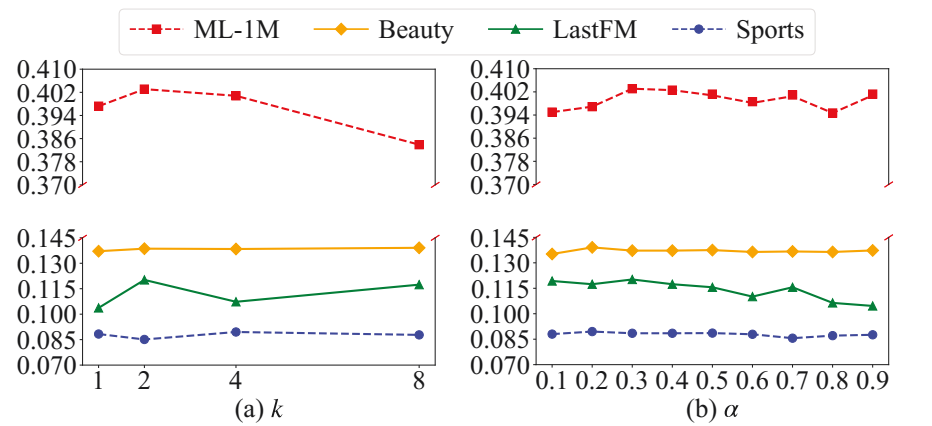
\includegraphics[width=\linewidth]{Hyper_parameter analysis.png}
    \caption{Visualization of the learned adaptive $\bm{G}$ and spectral changes in the FDFR module.}
    \label{fig:spectrum}
\end{figure}
\begin{figure}[t]
    \centering
    
    % 第一张图
    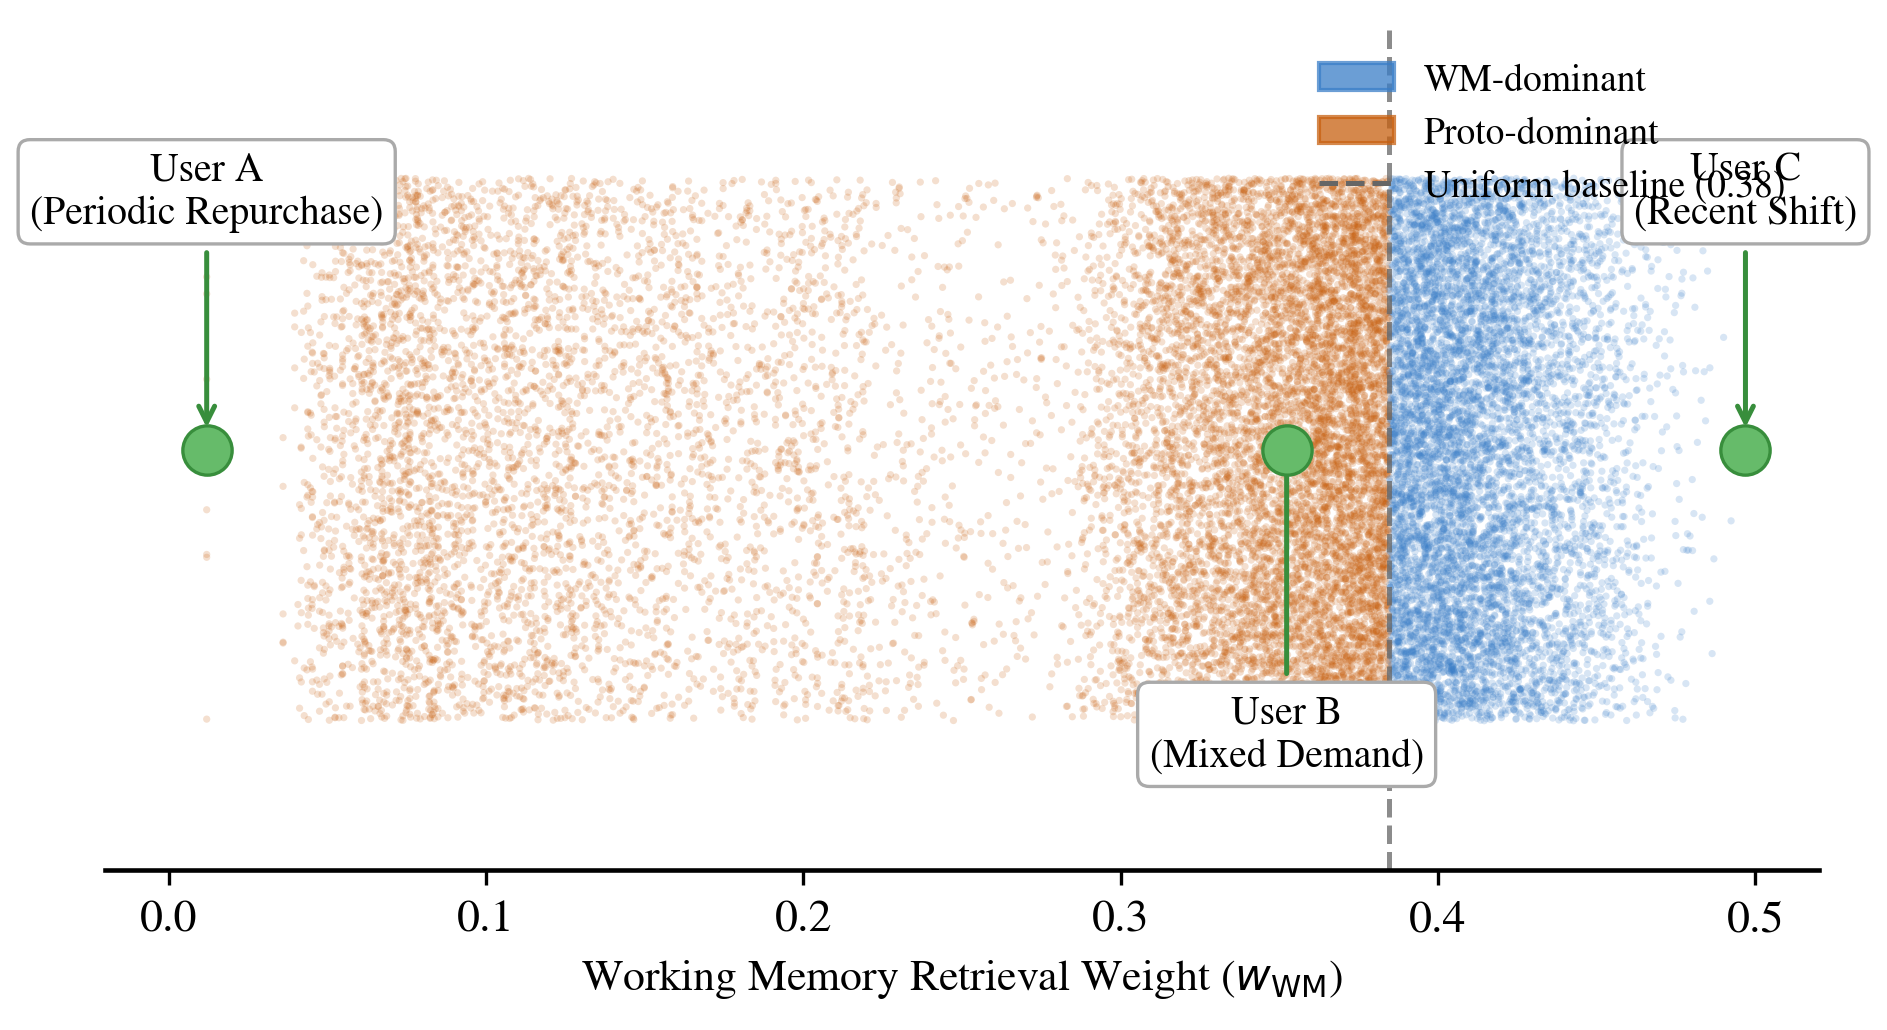
\includegraphics[width=\linewidth]{case1_final.png}
    \caption{Visualization of the learned adaptive $\bm{G}$ and spectral changes in the FDFR module.}
    \label{fig:spectrum}
\end{figure}


\subsection{Further Analysis}
\subsubsection{case1-final}
As shown in Table 2, DREAMRec consistently achieves the best performance across all datasets and evaluation metrics, demonstrating the effectiveness of the proposed user modeling framework. Compared with the strongest competing baseline, CCFRec, DREAMRec consistently improves both Recall and NDCG, indicating its ability to learn more accurate and discriminative user representations while generalizing well across datasets with different characteristics.
\subsubsection{case3-final}
As shown in Table 2, DREAMRec consistently achieves the best performance across all datasets and evaluation metrics, demonstrating the effectiveness of the proposed user modeling framework. Compared with the strongest competing baseline, CCFRec, DREAMRec consistently improves both Recall and NDCG, indicating its ability to learn more accurate and discriminative user representations while generalizing well across datasets with different characteristics.



\begin{figure}[t]
    \centering
    % 第一张图
    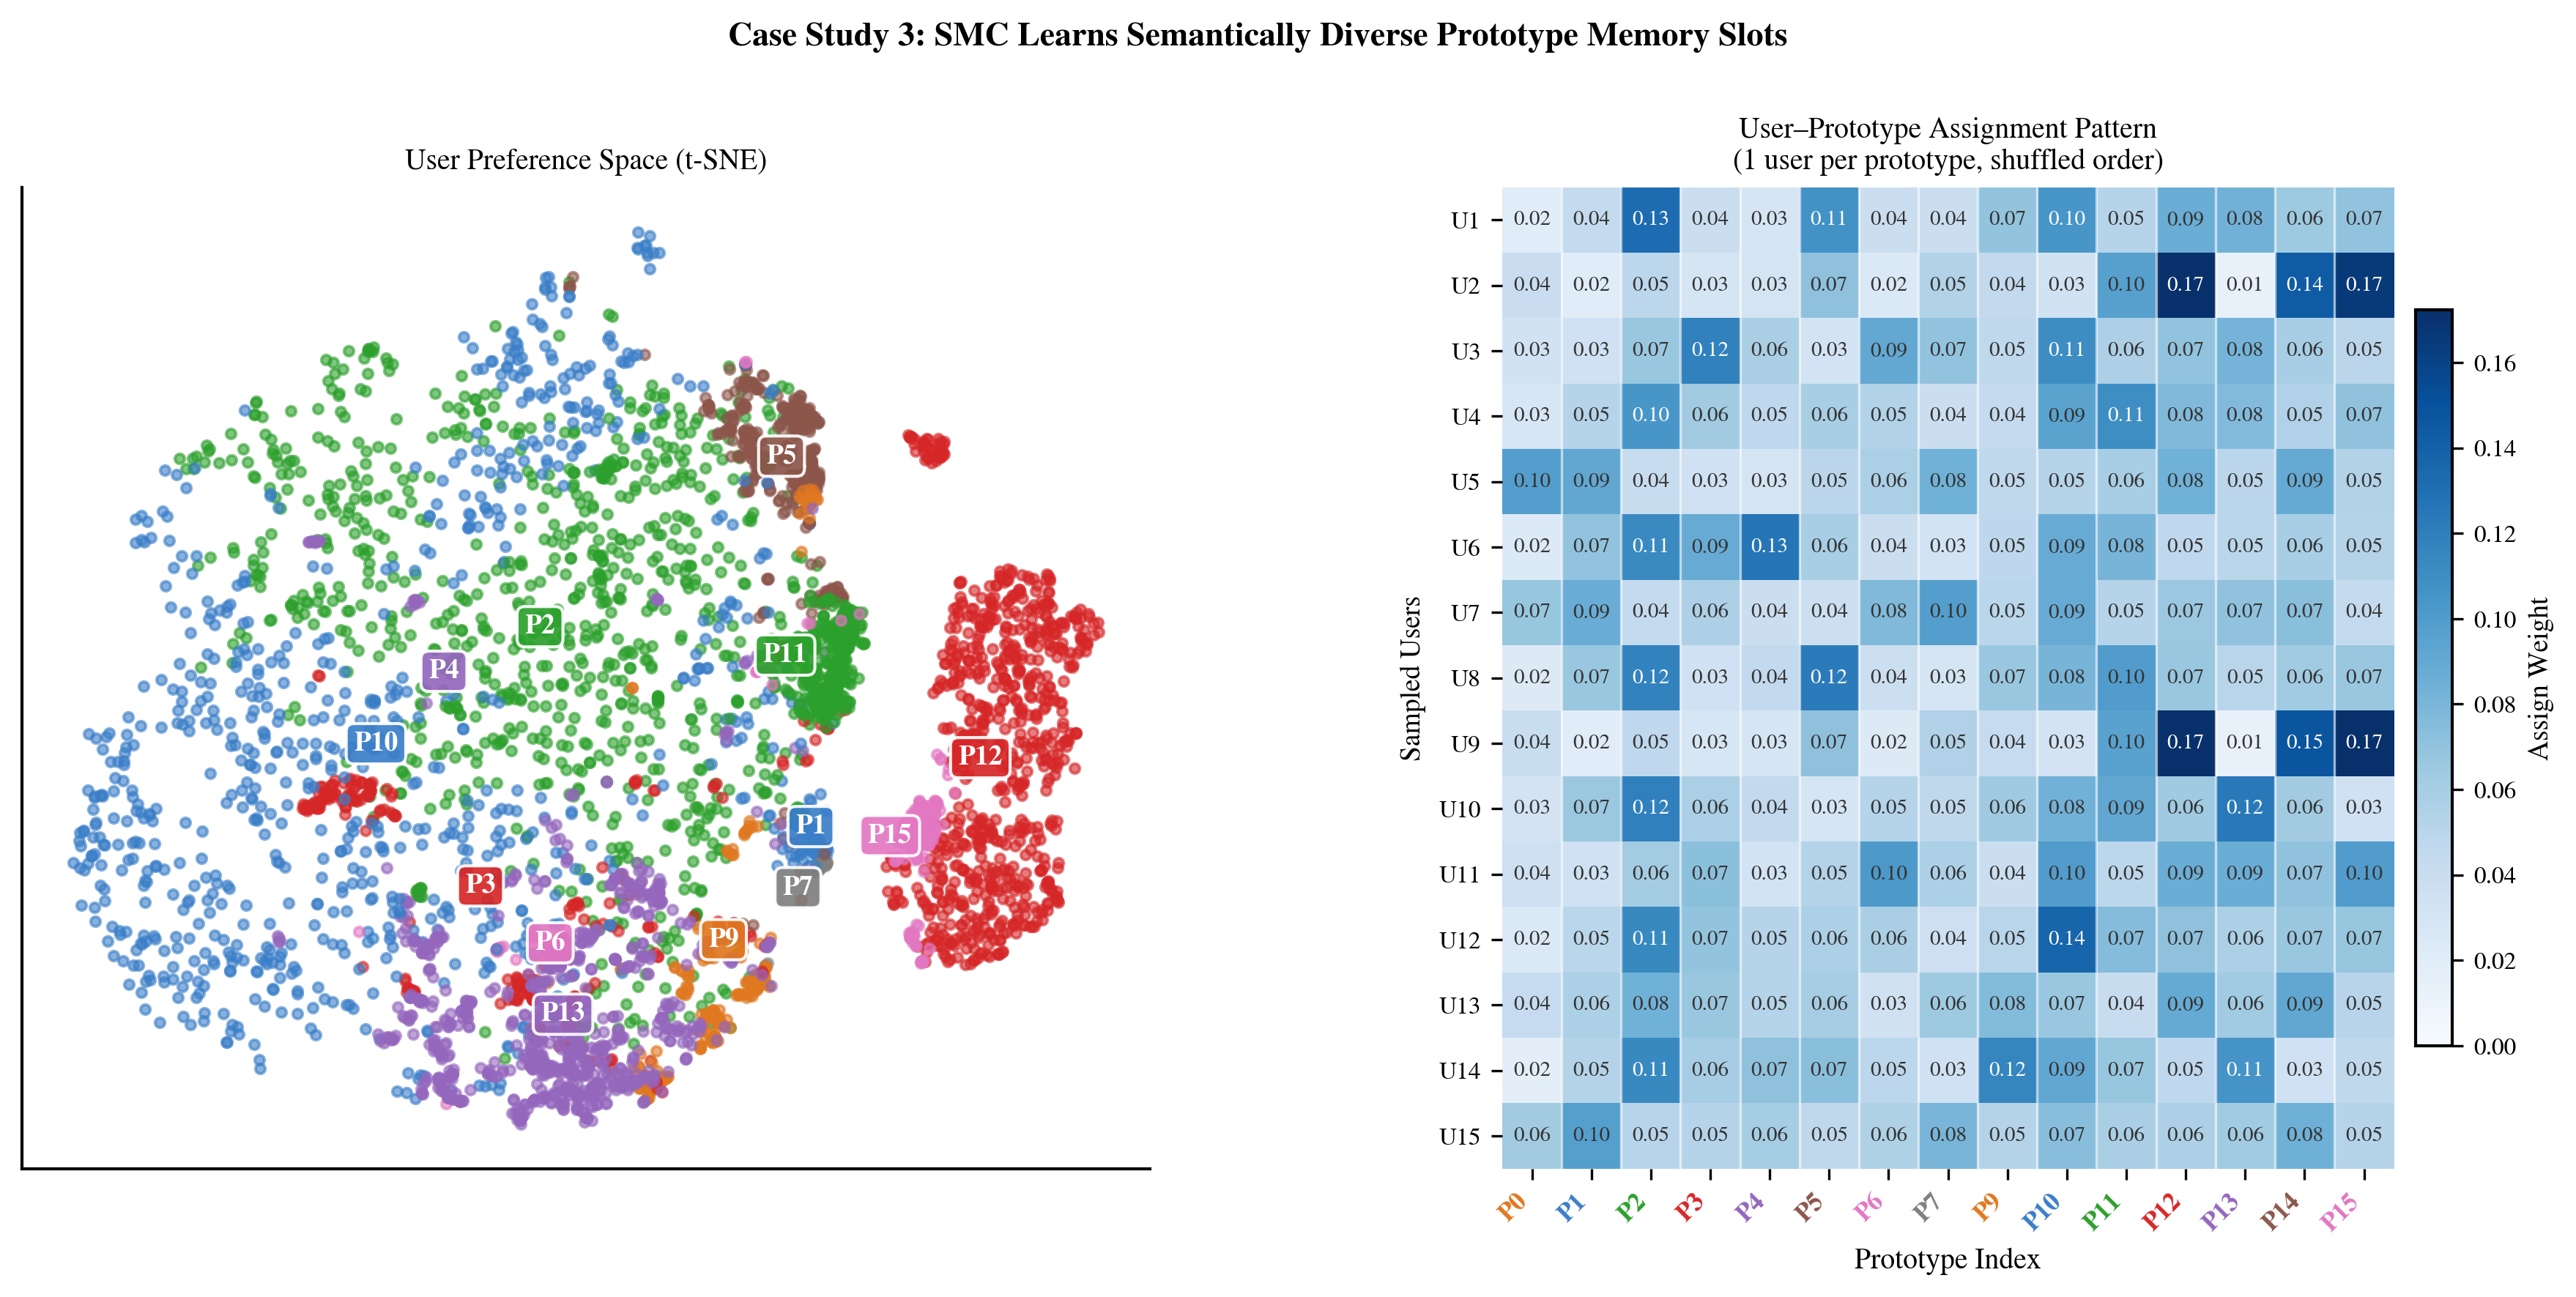
\includegraphics[width=\linewidth]{case3_final.png}
    \caption{Visualization of the learned adaptive $\bm{G}$ and spectral changes in the FDFR module.}
    \label{fig:spectrum}
\end{figure}


\subsection{Related work}
\subsubsection{case1-final}
As shown in Table 2, DREAMRec consistently achieves the best performance across all datasets and evaluation metrics, demonstrating the effectiveness of the proposed user modeling framework. Compared with the strongest competing baseline, CCFRec, DREAMRec consistently improves both Recall and NDCG, indicating its ability to learn more accurate and discriminative user representations while generalizing well across datasets with different characteristics.
\subsubsection{case3-final}
As shown in Table 2, DREAMRec consistently achieves the best performance across all datasets and evaluation metrics, demonstrating the effectiveness of the proposed user modeling framework. Compared with the strongest competing baseline, CCFRec, DREAMRec consistently improves both Recall and NDCG, indicating its ability to learn more accurate and discriminative user representations while generalizing well across datasets with different characteristics.

\subsection{conclusion}
As shown in Table 2, DREAMRec consistently achieves the best performance across all datasets and evaluation metrics, demonstrating the effectiveness of the proposed user modeling framework. Compared with the strongest competing baseline, CCFRec, DREAMRec consistently improves both Recall and NDCG, indicating its ability to learn more accurate and discriminative user representations while generalizing well across datasets with different characteristics.

\bibliography{aaai2027}

% Check whether the conference requires a reproducibility checklist to be included in the paper.
% If so, you can uncomment the following line and ajust the path to include it.
% \input{ReproducibilityChecklist.tex}

\end{document}
